\subsection{Skalarum}
Objekter i virkeligheden, såvel som detaljer i et billede, optræder kun som meningsfulde enheder over et specifikt skalainterval. Et simpelt eksempel er et træ, hvilket, indenfor meters afstand, vil opfattes som et træ, men indenfor centimeters eller nanometers afstand vil optræde som blade eller molekyler. I et billede vil de nærmeste objekter, optræde som fine strukturer og de længere væk, som grovere strukturer. 
\\
Formelt kan et billede repræsenteres som en funktion af to variable:
\begin{equation}
\begin{split}
&I: R^2 \rightarrow R \\
&I(x,y) = \lambda \hspace{0.5 cm} (x,y)\in R^2, \lambda \in R
\end{split}
\end{equation}
hvor $\lambda$ repræsentere en billedintensitet. Da billedet indeholder en ukendt scene, vides det ikke hvilket skalainterval, der for et givent objekt indgående i scenen, er meningsfuldt. En aksiomatisk tilgang til dette problem er at undersøge en bred skalarepræsentation af billedet i form af en udvidelse af billedfunktionen med en enkelt parameter også kaldt skalaparametren $\sigma$:
\begin{equation}
\begin{split}
&L: R^3 \rightarrow R \\
&L(x,y,\sigma) = \lambda \hspace{0.5 cm} (x,y,\sigma)\in R^3, \lambda \in R
\end{split}
\end{equation}
For at opnå en multi-skal repræsentation af billedet, oprettes der et skalarum bestående af skalabilleder, der går fra at fremhæve de finere strukturer til de grovere strukturer, proportionelt med skalaparametren som illustreret i figur \ref{fig:scalerep}. 
\begin{figure}[H]
    \centering
    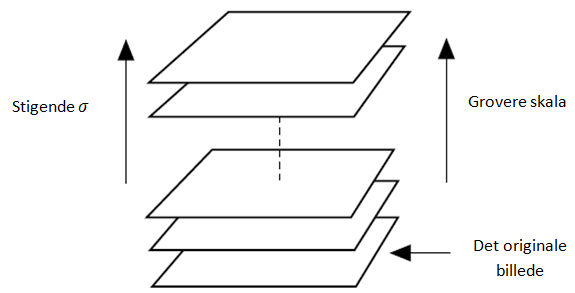
\includegraphics[width=0.45\textwidth]{fig/32.png}
     \vspace{-1em}
    \begin{center}    
       \caption{\textcolor{gray}{\footnotesize \textit{ }}}
    \label{fig:scalerep}
     \end{center}
     \vspace{-2.5em}
  \end{figure} \noindent
Denne overgang fra finere til grovere strukturer kan opnås ved iterativt at folde billederne med et Gaussisk filter af stigende $\sigma$ værdier:
\begin{equation}
L(x,y,\sigma) = G(x,y,\sigma)\ast I(x,y)
\label{scalespace1}
\end{equation}
, hvor billedets nulskala repræsenteres ved biledet $ L(x,y,0) = I(x,y)$. \\
Strukturer, der findes på grovere skalaer, må ikke være nyopståede objekter, men derimod simplificeringer af objekter eksisterende på de finere skalaer, hvilket tillades af det Gaussiske filter. Der anvendes et Gaussisk filter, på grund af dens unikke egenskaber,  bl.a. at der ikke forekommer nye strukturer ved glatning, når skalaparametren stiger. Witkins \cite{witkins} beviste dette i tilfældet for én-dimensionselle signaler som set i figur \ref{scalespace1}. Koenderink førte dette begreb videre til det to-dimensionelle tilfælde, ved at vise at enhver skalarum præsentation skal følge diffusions ligning, som beskriver hvordan en varmefordeling $I$ <plan> udvikler sig over tid $t$:
$$ \partial t I = \nabla^2I $$
Et lineært skalarum anvender en kontinuerlig stigende skalaparameter, der vedligeholder det samme skalainterval og niveau af glatning imellem skalaer.
Figur \ref{scalespace1} viser resultatet af at glatte et signal med et Gaussisk filter af stigende $\sigma$ værdi. Det ses tydeligt, hvordan signalets underliggende grovere struktur bliver fremhævet og at finere strukturer bliver fjernet.
\begin{figure}[H]
    \centering
    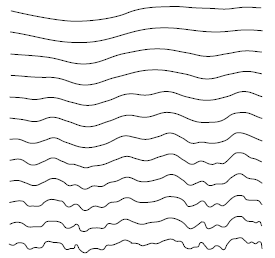
\includegraphics[width=0.45\textwidth]{fig/33.png}
     \vspace{-1em}
    \begin{center}    
       \caption{\textcolor{gray}{\footnotesize \textit{ }}}
    \label{fig:scalereps}
     \end{center}
     \vspace{-2.5em}
  \end{figure} \noindent
En anden, udbredt måde, at repræsentere et skalrum er ved en \textit{skalapyramide}.  